\chapter{基于GPU的极大二分团枚举并行实现}
\label{ch:gmbe}

针对现有极大二分团枚举算法在并行扩展性方面受限于CPU计算核心数量的问题,本章引入了具有大量计算核心的GPU作为计算资源,以加速极大二分团枚举过程。本章介绍了现代GPU的硬件架构和软件编程模型。同时,本章%整理了GPU加速图计算的相关工作,并
指出在GPU上实现极大二分团枚举所面临的挑战,作为研究的动机。具体而言,简单地将现有算法映射到大量的GPU计算核心中会遇到内存短缺、线程分歧和负载不均等问题。为了解决这些问题,本章提出了以下优化方法:首先,针对内存短缺问题,本章提出了基于枚举节点重用的迭代方法。该方法可以重用枚举树根节点内存,避免为新枚举节点动态分配内存,从而减少内存开销。其次,针对线程分歧问题,本章提出了局部邻居数量感知的剪枝方法。该方法通过记录枚举过程中顶点局部邻居数量的变化对枚举空间进行剪枝,缓解了线程分歧问题。然后,针对负载不均问题,本章提出了负载感知的任务调度方法。该方法将每棵子枚举树对应的计算任务与一个线程束的计算资源进行绑定,在运行时动态预估子枚举树的大小并对较大的子枚举树进行进一步拆分,实现了细粒度的负载均衡。最后,本章结合上述三种方法,提出了基于GPU的高效极大二分团枚举解决方案GMBE。实验证明,基于单个NVIDIA A100 GPU的GMBE相比现有基于96个CPU的并行算法ParMBE实现了70.6倍的性能提升。

\section{现代GPU架构与编程模型} 
\label{sec:gpu_arch}
GPU,即图形处理单元(Graphics Processing Unit),最初是专门用于处理图形数据的处理器。随着计算需求的增加,现代GPU逐渐演变成了通用并行处理器,能够高效执行大规模数据并行计算任务,如科学计算、深度学习和密码学等。与传统的中央处理器(Central Processing Unit,CPU)相比,现代GPU拥有更多的计算核心,并且能够利用这些核心并行处理大量数据,因此成为加速图计算的有力工具,同时具备加速极大二分团枚举问题的潜力。在本节中,我们将深入探讨现代GPU的硬件架构、与硬件架构对应的主流的软件编程模型CUDA (Compute Unified Device Architecture) 以及针对CUDA的编程指南,作为本章的研究背景。

\begin{figure} [t]
  \center
    % \vspace{0.1in}
		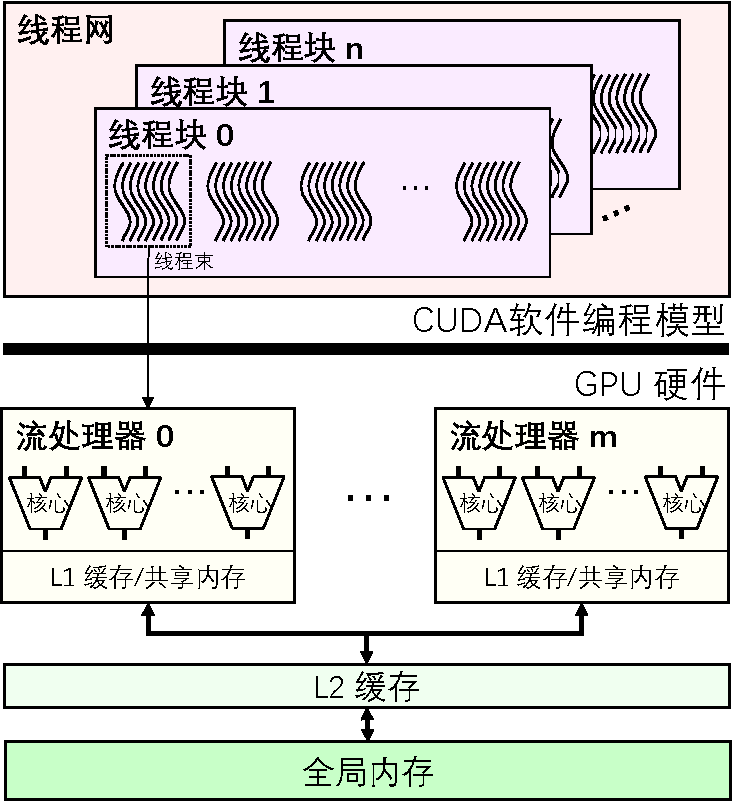
\includegraphics[width=0.55\linewidth]{gpu_arch}
     \vspace{-0.1in}
	\caption{现代GPU硬件架构与软件编程模型}
	\label{fig:gpu}
\end{figure}

图\ref{fig:gpu}展示了现代GPU的硬件架构和软件编程模型。GPU的\textbf{硬件架构}包括大量的计算核心,以及对应的层级存储结构。具体而言,一块现代GPU通常包括全局内存(Global Memory)、共享的L2缓存(Cache)以及大量的流处理器 (Streaming Multiprocessor, SM)。每个流处理器包含单独的L1缓存、可编程的具有多分区(Multi-bank)的共享内存(Shared Memory),以及多个轻量级计算核心(Core)。主流的GPU可以配备上万个轻量级计算核心,提供了巨大的计算能力。然而,与丰富的计算资源相比,GPU上的内存资源相对有限。例如,近年备受青睐的NVIDIA A100~\cite{NVIDIA-A100}最多可以提供6912个核心,但只能提供最多80GB的全局内存。

与GPU的多计算核心的硬件架构相对应,主流的\textbf{CUDA软件编程模型}按照层级结构管理大量线程。具体而言,CUDA编程模型提供了一个并行计算平台和一组API~\cite{CUDA-wiki,CUDAProgrammingGuide},允许用户高效地利用GPU进行通用目的的处理。CUDA采用SIMT (Single Instruction, Multiple Threads)~\cite{SIMT-wiki}执行模型来管理大量线程。它将GPU内核划分为多个线程网(Grid),每个线程网包含多个线程块(Block),每个线程块包括多个线程(Thread),并在执行期间分配给一个流处理器(SM)。流处理器将32个并行线程分组成一个线程束(Warp),并同时执行多个线程束。通过这种方式,成千上万个GPU核心可以高效地并行工作,实现高性能计算。




为了提升GPU的执行性效率,我们针对CUDA编程模型总结了\textbf{编程指南}如下:

\begin{figure} [t]
  \center
    % \vspace{0.05in}
		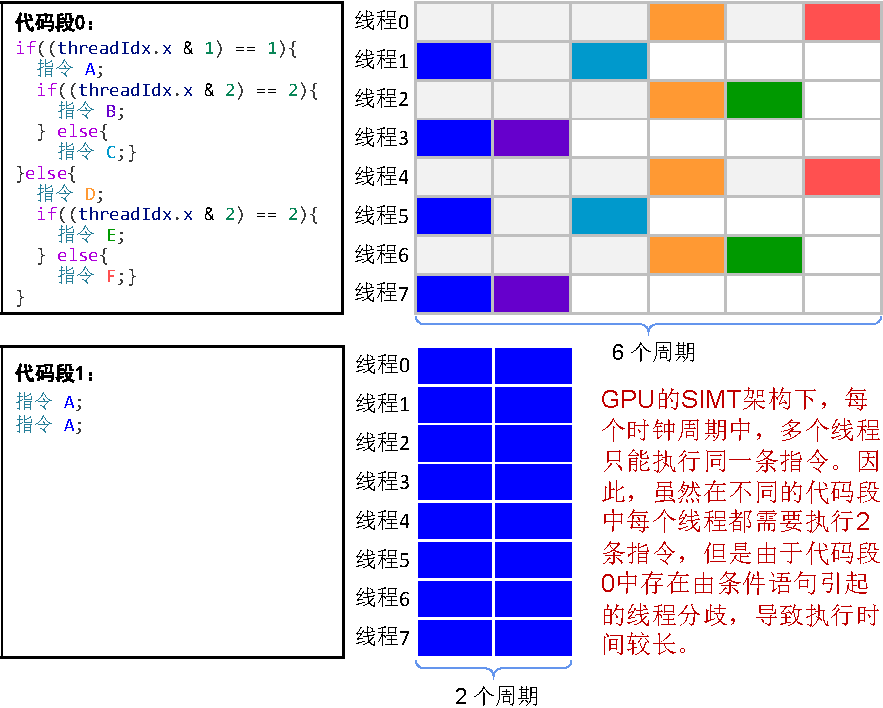
\includegraphics[width=0.8\linewidth]{gmbe/motivation_divergence}
    % \vspace{0.05in}
	\caption{线程分歧示意图}
	\label{fig:gmbe_motivation_divergence}
\end{figure}



\begin{enumerate}
  \item 减少动态内存分配。动态内存分配是指程序在运行过程中动态申请和释放内存。由于 GPU 允许大量的线程同时并发执行,大量线程可能会同时进行动态内存分配,从而引发线程争用、同步开销以及内存碎片化等问题,影响程序性能 ~\cite{DynamicMallocGpu21}。为了避免这种情况的发生,建议采用静态内存分配方式,在程序开始前预估程序的内存使用情况并一次性分配一块足够大的内存,然后在运行时重复使用这块内存,避免频繁的动态内存分配和释放,以降低内存管理的开销并优化内存访问效率。
  
  \item 减少线程分歧。线程分歧是指在 GPU 中同一线程束内的线程执行不同的代码路径。如图~\ref{fig:gmbe_motivation_divergence}所示,由于 GPU 使用 SIMT 的执行模式,即多个线程共享同一组指令,线程分歧会使 GPU 对不同执行路径进行串行化,导致部分线程处于空闲状态,从而严重影响执行性能 ~\cite{CUDAProgrammingGuide}。因此,在CUDA程序应设计简洁的算法和内核函数,尽量保持线程之间的执行路径相似,避免条件语句中大量的分支情况。可以考虑使用线程块内的协作和同步机制来避免线程分歧,尽量使每个线程束内的线程保持一致的执行路径,从而提高并行执行效率。
  

  \item 平衡大量负载。平衡大量负载是指合理地分配计算任务和数据处理任务,确保每个处理单元的负载均衡,避免某些处理单元负载过重而导致性能瓶颈。由于 GPU 拥有大量轻量级计算核心,负载不平衡会导致数千个计算核心等待最慢的计算核心执行,造成严重的资源浪费~\cite{CUDAProgrammingGuide}。为了实现负载平衡,可以考虑将任务划分为较小的子任务,并合理分配给不同的处理单元,通过动态调整任务分配策略来实现计算任务在不同计算资源上的均匀分布,从而提高整体计算效率。此外,可以利用CUDA提供的性能分析工具来帮助识别和解决负载不平衡的问题~\cite{Nsight,CUDANsightSystems,CUDANsightProfile},从而优化程序的性能表现。
  
\end{enumerate}


\section{研究出发点}

尽管GPU具有强大的并行能力,在部分图挖掘问题上已经显示出加速效果,但在GPU上实现高效的极大二分团枚举仍然面临严峻的挑战。具体而言,这些挑战主要包括的内存短缺、线程分歧和负载不均等。本节将结合GPU加速图计算的相关工作,对上述挑战进行详细说明。为了方便表述,本章中总是以算法~\ref{alg:se_mbe} 在二分图$G_3$上的集合枚举树为例,如图~\ref{fig:gmbe_tree}所示。

\begin{figure} [H]
	\centering
  \vspace{0.1in}
	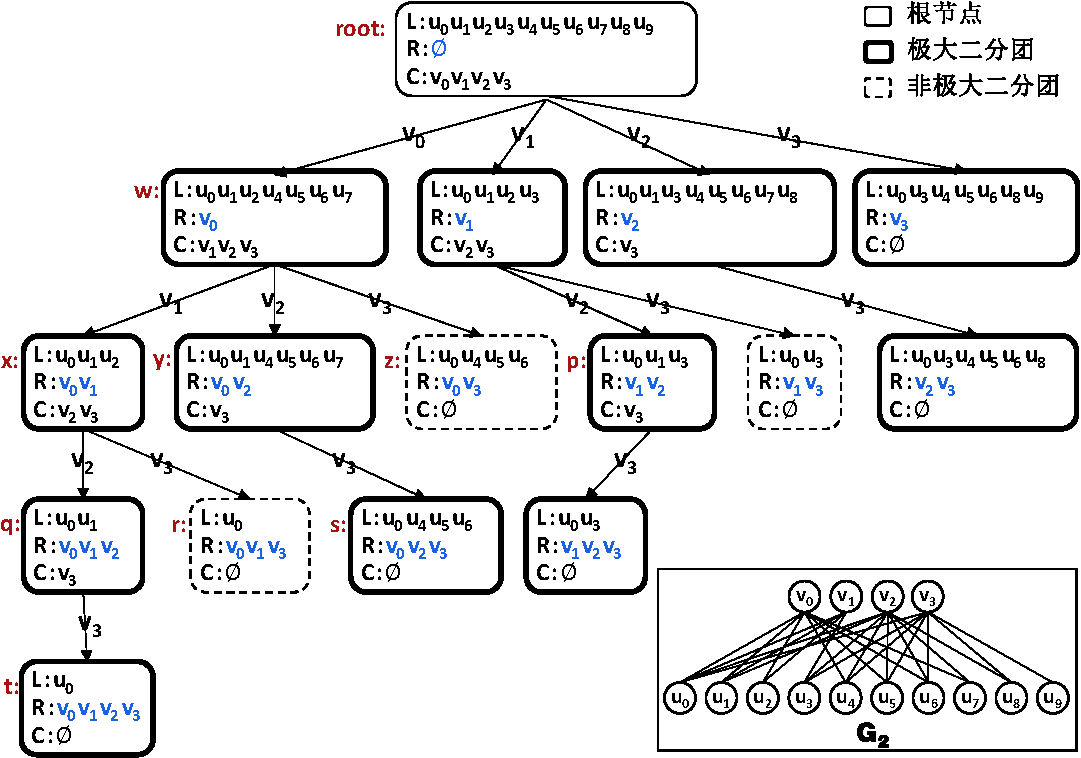
\includegraphics[width=0.9\linewidth]{gmbe/eg_tree}
  \vspace{0.1in}
	\caption{算法~\ref{alg:se_mbe}在二分图$G_3$上的集合枚举树}

	\label{fig:gmbe_tree}
\end{figure}

\subsection{内存短缺}
根据~\ref{subsec:algorithm}节的描述,我们注意到现有的极大二分团枚举算法(如算法~\ref{alg:se_mbe}所示)在枚举过程中会\emph{动态的生成和释放枚举节点$(L,R,C)$}。因此,直接将这类算法迁移到GPU上会导致~\ref{sec:gpu_arch}节中提到的动态内存分配问题。为了实现高性能,现有的基于GPU的图挖掘算法(例如~\cite{MCE-GPU21,Kclique22,g2miner22,Graphset23})通常在执行之前就在GPU上预先分配足够的内存空间来容纳所有的枚举节点。参考这些算法的内存估计方法,我们可以得出在极大二分团枚举算法中,每个枚举节点需要使用$O(|L|+|R|+|C|)$的内存,上限为$O(\Delta(V) + \Delta_2(V))$。同时,在遍历过程中,每棵子树最多需要保存$\Delta(V)$个活跃枚举节点用于回溯。因此,每棵枚举树的遍历过程需要预分配的内存总量为$\Delta(V) \times (\Delta(V) + \Delta_2(V))$ $\times$ \textit{顶点大小}。举例来说,在使用 NVIDIA A100 GPU(40 GB 内存)对真实世界的二分图 BookCrossing~\cite{konect} 进行极大二分团枚举时,每棵子树遍历过程的内存需求为$13,601 \times (13,601 + 53,915) \times$ \textbf{sizeof}(\textbf{int}) B = 3.67\,GB。为了充分利用NVIDIA A100 GPU中的108个流处理器 (SM), 我们需要$108 \times 3.67$ GB = 397 GB的内存,这超过了GPU中的内存空间 (40 GB),因此面临严重的内存短缺问题。

\subsection{线程分歧}
\label{subsec:gmbe_thread_divergence}

由于图挖掘算法本身的不规则性~\cite{Irregularity12},极大二分团枚举算法\emph{涉及大量的分支语句},这导致了~\ref{sec:gpu_arch}节所提到的线程分歧问题。在GPU上进行极大二分团枚举时,线程分歧主要来源于两个方面。首先,在极大二分团枚举过程中,同一线程束内的线程可能会同时访问不同的顶点以生成新节点,并使用不同顶点的邻居来计算不同的集合$L$、$R$和$C$,从而导致不同线程执行不同的控制流以访问不同内存区域。其次,如~\ref{sec:opt}节所述,现有的搜索空间优化方法通常会引入额外的判断语句来对搜索空间进行剪枝,导致不同线程执行路径差异,进一步加剧了线程分歧问题。举例来说,ooMBEA算法~\cite{ooMBE22} 需要访问所有候选顶点的2跳邻居来识别批量枢纽(Batch Pivots),并剪掉不属于批量枢纽的候选顶点,以实现剪枝目的。然而,访问顶点的2跳邻居需要进行深度为2的深度优先搜索,这个过程会涉及到大量对不同顶点邻居边界的条件判断,因而导致更严重的线程分歧问题。因此,在优化枚举空间的同时减少线程分歧是一项具有挑战性的任务,开发适用于GPU的剪枝方法至关重要。

\begin{figure} [H]
  \center
    \vspace{0.1in}
		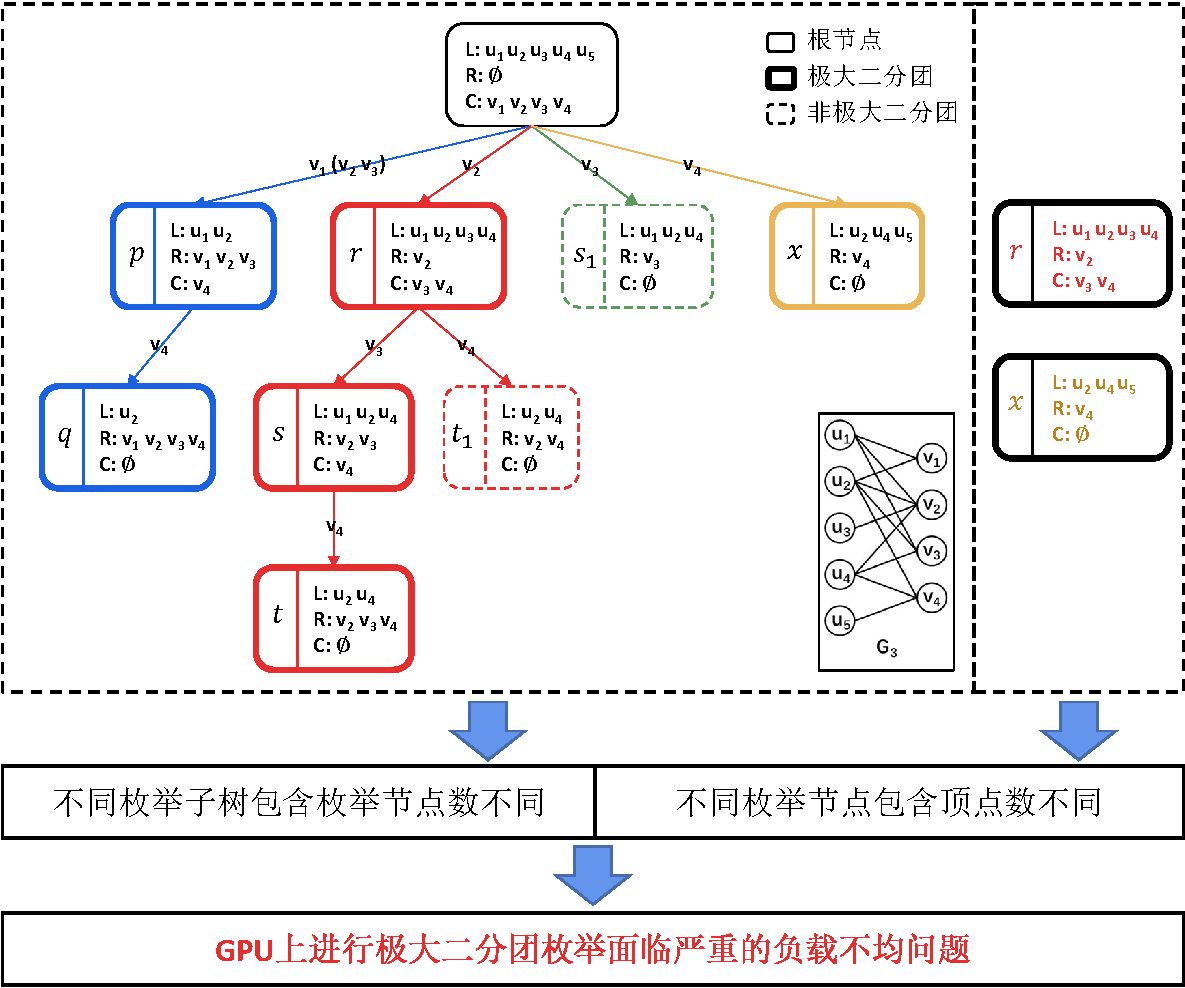
\includegraphics[width=0.85\linewidth]{gmbe/motivation_load}
    \vspace{0.1in}
	\caption{在GPU上进行极大二分团枚举中的负载不均问题说明}
	\label{fig:gmbe_load_reason}
\end{figure}


\subsection{负载不均}

如图~\ref{fig:gmbe_load_reason}所示,极大二分团枚举问题在GPU上面临严重的负载不均问题,这是由于\emph{不同子枚举树和枚举节点之间的计算差异性}所导致的。与其他GPU实现的图挖掘算法类似,我们将完整枚举树拆分成多个子枚举树,并尝试在不同计算单元之间平衡它们的负载分布~\cite{g2miner22,Kclique22,Graphset23}。我们没有选择按照更细粒度的枚举节点进行任务划分,因为在此类图挖掘问题中,枚举节点往往数量庞大,细粒度划分会增加任务调度的开销,严重降低整体性能。
目前,已有的图模式挖掘算法G$^2$Miner~\cite{g2miner22}通常将每个顶点生成的枚举子树分配给GPU上的一个线程束来独立执行。然而,我们的实验结果显示,这种粗粒度的GPU负载均衡策略在极大二分团枚举问题中效率较低。由于不同子枚举树包含的枚举节点数量差异很大,且每个节点内的顶点数量也不同,导致不同子枚举树的负载相差较大。这种负载不均会导致大量计算核心在等待最耗时的核心执行时浪费大量时间,造成资源的浪费。接下来,我们将通过一组实验结果详细说明这一问题。

% 根据图~\ref{fig:gmbe_load_reason}展示的情况,在GPU上运行的极大二分团枚举算法存在严重的负载不均问题,这是由于\emph{不同子枚举树和枚举节点之间的计算差异性}所导致的。负载不均会导致大量计算核心在等待最耗时的计算核心执行时浪费大部分时间,从而造成资源的浪费。目前,已有的图模式挖掘算法G$^2$Miner~\cite{g2miner22}通常将每个枚举子树分配给GPU上的一个线程束来独立执行。


\begin{figure} [H]
  \center
		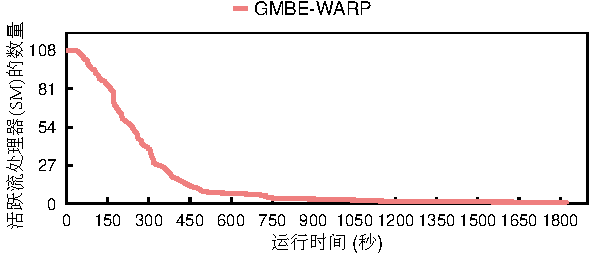
\includegraphics[width=0.7\linewidth]{gmbe/load_balance}
	\caption{在GPU上进行极大二分团枚举的负载不均问题示例}
	\label{fig:gmbe_load_example}
\end{figure}

\begin{example}

  图~\ref{fig:gmbe_load_example}展示了在简单负载均衡方案下,在GPU上进行极大二分团枚举表现出的负载不均问题。具体而言,首先,在我们的最终解决方案GMBE的基础上,我们应用G$^2$Miner算法中将每个顶点生成的枚举子树分配给GPU上的一个线程束来独立执行的任务调度方案,形成变种GMBE-WARP。随后,我们在BookCrossing数据集上运行GMBE-WARP,并记录了GPU内活跃流处理器数量随着运行时间的变化图。实验结果显示,该算法的总运行时间为1,822秒。当程序运行至20\%时(即364秒),活跃的流处理器仅有22个,占总数108个的20\%。这意味着在整个运行过程中,超过80\%的流处理器(86个SMs / 共108个SMs)将耗费80\%的运行时间(1,458秒 / 共1,822秒)等待最慢的一个子枚举树的计算。因此,现有的方法不能满足极大二分团枚举算法在GPU上的负载均衡需要,我们有必要实现更细粒度的负载均衡。
  
\end{example}


% 然而,如图~\ref{fig:gmbe_load_example}所示,如果简单采用我们提出的GMBE算法,将每个枚举树分配给一个线程束,将会导致大量资源浪费,影响性能。具体来说,该算法总共运行时间为1,822秒。当程序运行至20\%时(即364秒),活跃的流处理器仅有22个,占总数108个的20\%。这意味着在整个运行过程中,超过80\%的流处理器(86个SMs / 共108个SMs)将耗费80\%的运行时间(1,458秒 / 共1,822秒)等待最慢的一个子枚举树的计算。因此,对于MBE算法,有必要在更细粒度上平衡工作负载。


\section{GMBE算法设计与实现}
为了应对GPU上高效实现极大二分团枚举时所面临的内存短缺、线程分歧以及负载不均等挑战,本节提出了一系列对应的解决方案。这些解决方案包括基于枚举节点重用的迭代方法、局部邻居数量感知的剪枝方法以及负载感知的任务调度方法。最终,通过结合这些技术,我们提出了高效的GPU极大二分团枚举算法 GMBE。


\subsection{基于枚举节点重用的迭代方法}
\label{subsec:gmbe_memory}


为了减少内存使用,我们提出了一种基于枚举节点重用的迭代方法。该方法的核心思想在于仅保存子枚举树中的根节点$x$及其相关元数据,\textbf{在迭代过程中反复重用节点$x$的存储空间,避免为大量子节点动态分配空间}。在枚举过程中,后继节点总是能够从节点$x$的存储空间中获取,因为我们发现任何子节点$c$中的顶点集$L_c \cup R_c \cup C_c$始终是其父节点$x$的顶点集$L_x\cup R_x\cup C_x$的子集。例如,在图~\ref{fig:gmbe_tree}中,对于父节点$p$和子节点$q$,我们发现父节点$p$内的顶点集$\{u_1, u_2, v_1, v_2, v_3, v_4\}$包含子节点$q$内的顶点集$\{u_2, v_1, v_2, v_3, v_4\}$,这种父子节点间顶点集间普遍存在的包含关系为枚举节点重用技术提供了理论保证。接下来,我们在图~\ref{fig:gmbe_node_buf}中给出了基本的根节点存储结构,并结合算法~\ref{alg:gmbe_stack}详细描述了基于枚举节点重用的迭代方法。



% 在枚举过程中,我们总是能够实现枚举节点重用,因为我们观察到节点$x$的子节点的$L\cup  R\cup C$总是其父节点$x$的$L\cup  R\cup C$的子集。例如,在图~\ref{fig:gmbe_load_example}中,我们可知子节点$q$ $(\{u_2\},\{v_1, v_2, v_3, v_4\}, \emptyset)$ 中的顶点$\{u_1, u_2, v_1, v_2, v_3, v_4\}$ 是其父节点$p$ $(\{u_1, u_2\}, \{v_1, v_2, v_3\},\{v_4\})$ 中顶点的子集。算法~\ref{alg:gmbe_stack}具体描述了基于枚举节点重用的迭代方法。

\begin{figure} [H]
  \center
    % \vspace{-0.1in}
    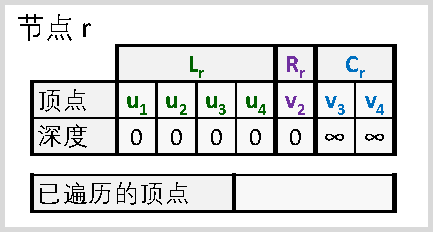
\includegraphics[width=0.4\linewidth]{gmbe/eg_node_buf}
    % \vspace{0.1in}
  \caption{$node\_buf$结构示意图}
  \label{fig:gmbe_node_buf}
\end{figure}


\begin{algorithm} [H]
  \begin{algorithmic}[1]
    \normalsize
    \REQUIRE 二分图 $G(U,V,E)$
    \ENSURE 所有极大二分团
    
    \renewcommand{\algorithmicwhile}{\textbf{procedure}}
    \renewcommand{\algorithmicdo}{\textbf{:}}
    \STATE \textsf{iteratively\_search}$(U,\emptyset,V)$;

    \WHILE{\textsf{iteratively\_search}$(L_r,R_r,C_r)$}
    \renewcommand{\algorithmicwhile}{\textbf{while}}
    \renewcommand{\algorithmicdo}{\textbf{do}}
      \STATE $node\_buf$ \textsf{.init\_and\_push}$((L_r,R_r,C_r))$;
      \WHILE{$node\_buf$非空}
        \STATE $(L_p, R_p, C_p) \leftarrow node\_buf$\textsf{.pop}$()$;
        \IF{$C_p$非空}
          \STATE $v' \leftarrow C_p$ 中编号最小的顶点; 
          \STATE $node\_buf$\textsf{.push}$((L_p,R_p,C_p \setminus \{v'\} ))$;
          \STATE $L' \leftarrow L_p \cap N(v');$ $R'\leftarrow R_p;$ $C' \leftarrow \emptyset$;
          \FOR{$v_c \in C_p$}
            \IF{$L' \cap N(v_c) = L'$}
              \STATE $R' \leftarrow R' \cup \{v_c\}$;
            \ELSIF{$L' \cap N(v_c) \neq \emptyset$}
              \STATE $C' \leftarrow C' \cup \{v_c\}$;
            \ENDIF
          \ENDFOR
          \IF{$R' = \Gamma(L')$}
            \STATE 输出极大二分团$(L', R')$;
            \STATE $node\_buf$\textsf{.push}$((L',R',C'))$;
          \ENDIF
        \ENDIF
        
      \ENDWHILE
    \ENDWHILE

  \end{algorithmic}
  \caption{基于枚举节点重用的MBE迭代算法}
  \label{alg:gmbe_stack}
\end{algorithm}


具体而言,我们不再以递归的方式创建和释放枚举节点,而是采用类似栈的结构$node\_buf$进行显式的迭代 。如图~\ref{fig:gmbe_node_buf}所示,每个$node\_buf$包括根节点内的所有顶点、每个顶点的深度属性、以及从根节点到当前节点所遍历的所有顶点。每个\textit{顶点}的\emph{\textit{深度}}根据当前节点的\emph{祖先节点数量}确定。\textit{已遍历的顶点}记录着从子枚举树根节点到当前节点所遍历的顶点,用于回溯搜索。在枚举过程中,我们只需要主动更新\textit{顶点}的\textit{深度}属性以及记录\textit{已遍历的顶点}。通过这种方式,迭代过程可以重用$node\_buf$对应的固定内存区域推导出所有的后继节点,进而极大程度地减少了GPU中的内存开销。算法~\ref{alg:gmbe_stack}首先用根节点初始化$node\_buf$(第3行)。随后算法迭代地获取$node\_buf$中的当前节点$(L_p,R_p,C_p)$(第5行)。如果当前节点的候选顶点非空,则迭代地选择当前节点内其中的一个候选顶点产生新的枚举节点(第6-21行),否则弹出该节点,继续迭代流程。最终,算法与递归算法~\ref{alg:se_mbe}得到相同的计算结果。接下来,我们将详细阐述涉及枚举节点重用的关键函数:


\begin{itemize}
  \item  \textsf{init\_and\_push}$((L_r,R_r,C_r))$ : 该函数用于利用子树的根节点$(L_r,R_r,C_r)$创建并初始化$node\_buf$ (第3行)。$node\_buf$存储了$L_r \cup R_r \cup C_r$中的所有顶点,并记录每个顶点的深度以及已遍历的顶点。我们将$L_r \cup R_r$中顶点的深度初始化为0,将$C_r$中顶点的深度初始化为$\infty$。
  
  \item  \textsf{push}$((L',R',C'))$ : 该函数用于向$node\_buf$中压入一个新的子节点$(L',R',C')$ (第8,20行)。首先,根据顶点深度的定义,我们知道当前节点的深度D总是比$node\_buf$中已遍历的顶点多一个。当我们在深度为D处压入一个新节点$(L',R',C')$时,我们知道$L' \subset L_r$, $R' \subset R_r \cup C_r$ 且 $C' \subset C_r$。我们将$L'$内顶点的深度更新为D,$R'$内深度为$\infty$的顶点的深度更新为D。因此,通过访问顶点的深度属性,我们总是能够在原始的$(L_r,R_r,C_r)$对应的$node\_buf$中找到新节点$(L',R',C')$,其中$L'$包含$L_r$内所有深度为D的顶点,$R'$包含$R_r\cup C_r$中所有深度不大于D的顶点,$C'$包含$C_r$中深度为$\infty$的顶点。最后,我们将用于生成节点$(L',R',C')$的已遍历顶点加入到已遍历的顶点集中。

  \item  \textsf{pop}$()$ : 该函数用于得到当前栈顶节点$(L_p,R_p,C_p)$,并利用$node\_buf$回溯到其父节点 (第5行)。当我们在节点深度D处弹出节点$(L_p,R_p,C_p)$时,首先移除已遍历的顶点集中最新遍历的顶点,然后将$L_p$内顶点的深度更新为D-1,将$C_r$内深度为D的顶点的深度更新为$\infty$。
  
\end{itemize}




与传统的单一记录节点内顶点的枚举树节点结构相比,我们提出的$node\_buf$在单个节点上额外记录了顶点\textit{深度}以及\textit{已遍历的顶点},其内存开销的上限为$3 \times \Delta(V) + 2 \times \Delta_2(V)$。但是与传统方法需要动态产生和释放枚举节点不同,$node\_buf$结构能够在枚举过程中被所有后继枚举节点重复使用,因此显著减少了遍历每棵枚举树的内存需求,为在GPU上并发运行数千个极大二分团枚举过程提供可能。例如,一块拥有40 GB内存的A100 GPU足以在BookCrossing数据集上并发运行超过10,000个子枚举树枚举过程,因为每个过程仅需要$(3 \times 13,601 + 2 \times 53,915) \times$ \textbf{sizeof}(int) B = 595 KB。与传统的方法相比,后者需要$13601 \times (13,601 + 53,915)\times$ \textbf{sizeof}(int) B = 3.67 GB,这种枚举节点重用方法在BookCrossing上的内存使用减少了6,178倍。

\subsection{局部邻居数量感知的剪枝方法}
\label{subsec:gmbe_prune}

现有的剪枝方法在GPU上由于线程分歧导致效率较低。为了解决这一问题,我们提出了一种新的剪枝方法,旨在减少枚举空间的同时减少线程分歧。具体而言,参照表~\ref{tab:definition},对于给定节点$(L, R, C)$,我们将顶点$v \in V$的\emph{局部邻居}定义为$N_L(v)$,其中$N_L(v)$等于$N(v) \cap L$。随后,我们定义\emph{局部邻居数量}为局部邻居的顶点个数。在算法~\ref{alg:gmbe_stack}中,候选顶点的局部邻居数量总是作为中间结果出现 (第11、13行),因此,我们能够在不引入额外计算的情况下得到候选顶点的局部邻居数量。基于这一现象,我们总结了如下定理:

\begin{theorem}
  假设当前节点为枚举树中的节点$s$,在选择候选顶点$v_r$时,如果对于当前节点$s$中顶点$v_r$的局部邻居数量与任一子节点$t$中顶点$v_r$的局部邻居数量相等,我们可以安全地裁剪由节点$s$选择顶点$v_r$所产生的子节点。
  \label{theorem:gmbe_prune}
\end{theorem}

\begin{proof}
  为了证明该定理,我们假设节点$s$已经遍历顶点$v_t$产生节点$t$,并且节点$s$将遍历顶点$v_r$产生新的节点$r$。进一步地,我们假设节点$s$中顶点$v_r$的局部邻居数量与子节点$t$中顶点$v_r$的局部邻居数量相等,即$N(v_r) \cap L_s =N(v_r) \cap L_t$。由于$L_t = L_s\cap N(v_t)$,我们知道$N(v_r) \cap L_s =N(v_r) \cap L_t= N(v_r) \cap L_s\cap N(v_t)$,因此$N(v_r) \cap L_s \subseteq N(v_t)$。由于$L_r = N(v_r)\cap L_s$,我们知道$L_r\subseteq N(v_t)$,即$v_t$与$L_r$中的所有顶点相连。由于我们已经遍历$v_t$产生节点$t$,因此节点$r$无法使用$v_t$扩展$R_r$,进而产生非极大二分团。因此我们可以安全地裁剪节点$r$。

\end{proof}

根据定理~\ref{theorem:gmbe_prune},我们观察到可以通过比较父子节点中候选顶点局部邻居数量是否变化进行剪枝。因此,在算法~\ref{alg:gmbe_stack}中,我们通过在$node\_buf$中额外维护所有候选顶点的局部邻居数量来进一步优化。具体而言,在$node\_buf$执行弹出操作\textsf{pop()}弹出节点$r$时,会临时保存栈顶节点候选顶点的局部邻居数量。当恢复到节点$r$的父节点$p$时,我们将对节点$p$和节点$r$中候选顶点的局部邻居数量进行批量比较。如果发现部分候选顶点的局部邻居数量未发生变化,我们可以安全地裁剪这些无用顶点。相比现有剪枝方法中涉及大量判断语句所引入的线程分歧问题,这种剪枝方法在GPU上不会额外引入线程分歧问题,因为剪枝的过程同一线程束中的线程总是批量比较相同候选集中的元素。我们通过一个示例详细展示了基于栈的迭代算法,并利用局部邻居数量进行剪枝。





% 根据定理~\ref{theorem:gmbe_prune},我们观察到可以通过比较父子节点中候选顶点局部邻居数量是否变化进行剪枝。因此,在算法~\ref{alg:gmbe_stack}中,我们通过在$node\_buf$中额外维护所有候选顶点的局部邻居数量来进一步优化。如果在弹出一个已遍历的子节点后,候选顶点的局部邻居数量保持不变,我们便可以裁剪这些无用的候选顶点。这种新的剪枝方法具有较低的线程分歧,因为同一线程束中的线程总是批量比较相同候选集中的元素。我们通过一个示例详细展示了基于栈的迭代算法,并利用局部邻居数量进行剪枝。







\begin{figure} [H]
  \center
    \vspace{0.1in}
		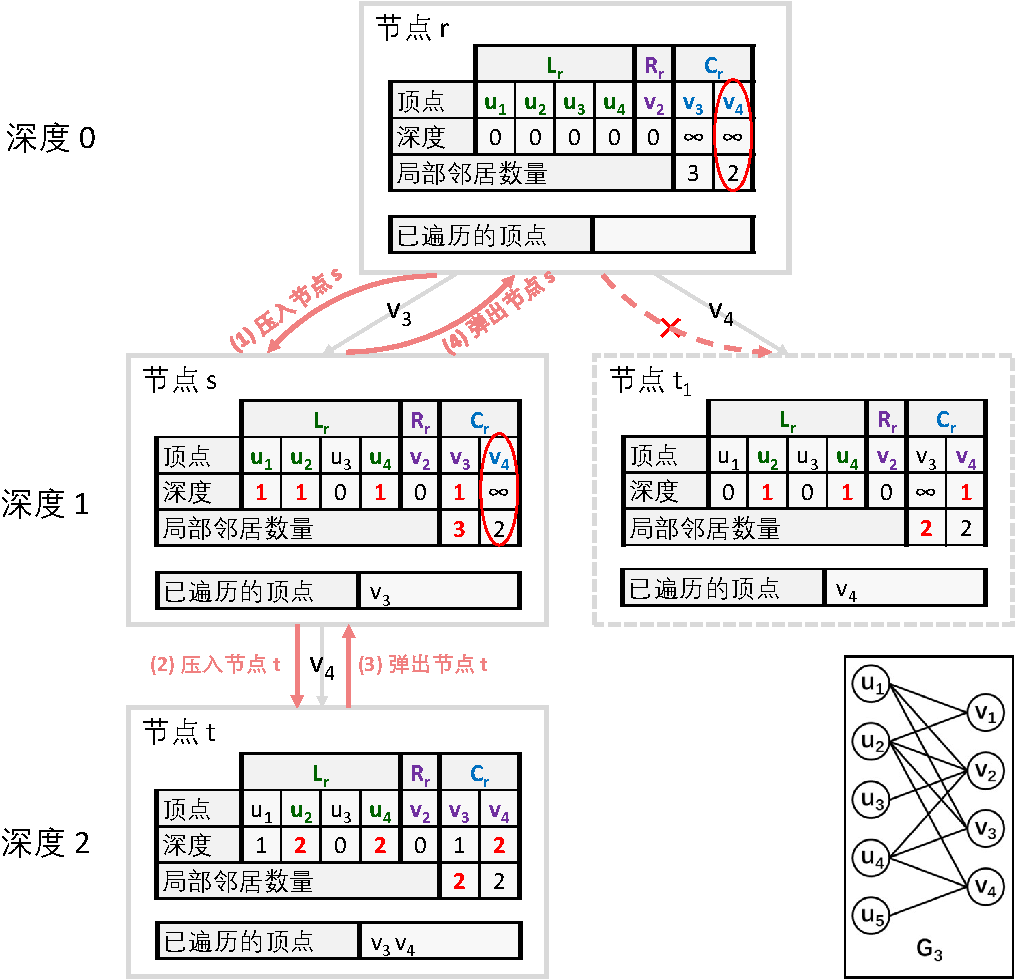
\includegraphics[width=0.8\linewidth]{gmbe/eg_prune}
    \vspace{0.1in}
	\caption{基于局部邻居数量的剪枝方法示意图}
	\label{fig:gmbe_prune}
\end{figure}

\begin{example}
  如图~\ref{fig:gmbe_prune}所示,在图~\ref{fig:gmbe_tree}中以节点$r$为根节点的子树中,算法利用$node\_buf$中固定大小的内存,迭代地枚举了其中的所有极大二分团。具体而言,我们首先使用节点 r $(L_r, R_r, C_r)$初始化$node\_buf$,将$L_r \cup R_r$中的顶点深度初始化为0,并将$C_r$中的顶点深度初始化为$\infty$。对于$C_r$中的顶点,$node\_buf$根据定义初始化了其局部邻居数量(即$|N_L|$)。例如,在节点$r$处,我们初始化$v_3$的局部邻居数量$|N_L(v_3)|$为$|N(v_3) \cap L_r| = 
  |\{u_1, u_2, u_4\}\cap \{u_1,u_2,u_3,u_4\}| = 3$。

  接下来,我们通过遍历$v_3$生成了节点$s$。我们知道$L_s=L_r\cap N(v_3)=\{u_1, u_2, u_4\}$。节点$s$的深度为1,$node\_buf$将$L_s\cup R_s$中顶点$u_1, u_2, u_4,$ 和 $v_3$的深度更新为1。其他顶点的深度保持不变。随后,我们利用$L_s$更新了$v_3$和$v_4$的局部邻居数量。通过计算,我们知道$|N_L(v_3)|$ = $|N(v_3) \cap L_{(s)}|$
  = $|\{u_1, u_2, u_4\} \cap \{u_1, u_2, u_4\}|$ = 3。
  $|N_L(v_4)|$ = $|N(v_4) \cap L_{(s)}|$
  = $|\{u_2, u_4, u_5\} \cap \{u_1, u_2, u_4\}|$ = 2。我们可以类似地生成其他节点。

在处理完以节点$s$为根节点的子树后,$node\_buf$弹出节点$s$并重置顶点的深度和局部邻居数量,用于恢复节点$r$。对于$node\_buf$内深度与节点$s$深度相同的顶点,我们将$u_1$,$u_2$和$u_4$的深度重置为0,并将$v_3$的深度重置为$\infty$。由于弹出节点$s$后,$v_4$的局部邻居数量始终是2,我们主动地在节点$r$处通过移除无用的候选顶点$v_4$来进行剪枝。


\end{example}


\subsection{负载感知的任务调度方法}
\label{subsec:gmbe_design_load}

为了进一步探索极大二分团枚举任务在GPU上的大规模并行性,我们提出了负载感知的任务调度方法。在图挖掘算法的GPU上任务调度方面,一种简单的方法是为每个子枚举树分配一个任务。如算法~\ref{alg:gmbe_task_naive}所示,我们用集合$V$中的不同顶点$v_s$产生不同的枚举子树,分别作为一个任务。

\begin{algorithm} [H]
  \begin{algorithmic}[1]
    \normalsize
    
    \FOR{$v_s \in V$}
      \STATE $L_s \leftarrow N(v_s); R_s\leftarrow\{v_s\}; C_s\leftarrow \emptyset $;
      \FOR{$v_c \in N_2(v_s)$}
        \IF{$L_s \cap N(v_c) = L_s$}
          \STATE $R_s \leftarrow R_s \cup \{v_c\}$;
        \ELSIF{$v_c$的索引在$v_s$之后}
          \STATE $C_s \leftarrow C_s \cup \{v_c\}$;
        \ENDIF 
      \ENDFOR

      \IF{$v_s$是$R_s$中索引最小的顶点}
        \STATE \textsf{iteratively\_search}$(L_s,R_s,C_s)$;
      \ENDIF

    \ENDFOR

  \end{algorithmic}
  \caption{GPU任务调度的简单方法}
  \label{alg:gmbe_task_naive}
\end{algorithm}


然后,我们可以参考已有的图挖掘算法,将每个任务映射到GPU的不同的线程束~\cite{g2miner22}或者不同线程块~\cite{Kclique22}上。我们将两种方案分别称为\textit{基于线程束的调度方法(Warp-centric Scheme)}和\textit{基于线程块的调度方法(Block-centric Scheme)}。然而,我们的研究表明,由于算法~\ref{alg:gmbe_task_naive}在第11行创建的并行任务运行时间差异很大,对于极大二分团问题,这两种简单的调度方法不足以平衡GPU中不同流处理器 (SM)上的任务负载。具体而言,在一个线程束或一个线程块中运行的最慢任务经常阻塞其他任务,导致EuAll数据集上高达97.8\%的性能下降。~\ref{subsec:gmbe_breakdown}节将展示更多任务调度相关的实验结果。




为了更好地平衡GPU中的任务负载,我们提出了一种针对极大二分团枚举的\textit{负载感知的基于任务的调度方法(Task-centric Scheme)}。该方法基于GPU编程模式中的持久线程编程模型(Persistent Thread, PT)~\cite{PersistentThread12}。具体而言,我们根据GPU中的流处理器数量创建对应数量的线程组,将每个线程组固定地映射到一个GPU的流处理器上。随后,为每个线程组设置固定数量的线程束,将每个流处理器上线程束的数量用\textit{WarpPerSM}表示,并在后文讨论其对系统性能的影响。



我们设计了一个可以创建负载感知任务的GPU核函数(Kernel Function),该函数会将处理较大枚举树的任务递归地分解为更小的任务,并将这些负载感知任务添加到每个流处理器的全局结构\textit{SM\_task\_queue}中。当一个任务完成时,PT的软件调度器会从\textit{SM\_task\_queue}中出队一个任务,并在相应的SM上迭代执行\textsf{}{iteratively\_search()}。

为实现负载感知,关键问题在于高效地检测出哪些负载的任务较重,并及时对高负载任务进行分解。对此,我们根据子枚举树根节点$(L,R,C)$的信息来估计枚举树的高度和节点数量。具体而言,我们估计枚举树的高度为$\min\{|L|,|C|\}$。我们估计枚举树中节点数量为$\min\{|L|,|C|\}\times|C|$,因为$|C|$代表了每个节点能够产生子节点的最大数量。我们经验性地设置了两个阈值$bound\_height$ 和 $bound\_size$,只有当$\min\{|L|,|C|\}$大于$bound\_height$且$\min\{|L|,|C|\}\times|C|$ 大于 $bound\_size$时,我们将该任务分解成多个子任务,以实现更好地负载平衡。

算法~\ref{alg:gmbe_task_full}描述了针对极大二分团枚举问题的GPU负载感知的基于任务的调度算法。当\textit{SM\_task\_queue}不为空时,它从队列里获取一个节点(第6行),如果我们估计该节点对应的负载较小时,我们直接启动一个GPU任务(第37行);反之,如果对应的负载超过阈值时(第23行),我们将该任务拆分成小任务并将小任务对应的根节点入队进行枚举(第23-35行)。这些小任务对应的节点将重新参与\textit{SM\_task\_queue}的调度。如果\textit{SM\_task\_queue}为空时,我们将从$processing\_v$获取需要处理的当前顶点$v_s$。然后用顶点$v_s$产生一个枚举任务,并运行在GPU上(第8-20行)。

\begin{algorithm} [H]
  \begin{algorithmic}[1]
    \normalsize

    \STATE $processing\_v$是一个全局变量,初始化为0;
    \STATE $SM\_task\_queue$是用于负载均衡的全局并发队列 ;
  
    \renewcommand{\algorithmicwhile}{\textbf{procedure}}
    \renewcommand{\algorithmicdo}{\textbf{:}}

    \WHILE{\textsf{warp\_kernel}}
    \renewcommand{\algorithmicwhile}{\textbf{while}}
    \renewcommand{\algorithmicdo}{\textbf{do}}
      \WHILE{\textbf{true}}
        \IF{$SM\_task\_queue$非空}
          \STATE $(L,R,C) \leftarrow SM\_task\_queue$\textsf{.dequeue}$()$ ;
        \ELSE
          \STATE $v_s$ = \textsf{atomicInc}$(processing\_v)$
          \IF{$v_s \in V$}
            \STATE $L \leftarrow N(v_s); R\leftarrow\{v_s\}; C\leftarrow \emptyset $;
            \FOR{$v_c \in N_2(v_s)$}
              \IF{$L\cap N(v_c) = L$}
                \STATE $R \leftarrow R \cup \{v_c\}$;
              \ELSIF{$v_c$的索引在$v_s$之后}
                \STATE $C \leftarrow C \cup \{v_c\}$;
              \ENDIF
            \ENDFOR
          \ELSE
            \STATE \textbf{return};
          \ENDIF
        \ENDIF

        \IF {$R = \Gamma(L)$}
          \IF {$\min\{|L|,|C|\}\times|C| >$ 数量边界,并且$\min\{|L|,|C|\} >$ 高度边界 }
            \FOR{$v_t \in C$}
              \STATE $L_t \leftarrow N(v_t); R_t\leftarrow R; C_t\leftarrow \emptyset $;
              \FOR{$v_c \in C$}   
                \IF {$L_t \cap N(v_c) = L_t$}
                  \STATE $R_t \leftarrow R_t \cup \{v_c\}$;
                \ELSIF{$L_t \cap N(v_c)$ 非空}
                  \STATE $C_t \leftarrow C_t \cup \{v_c\}$;
                \ENDIF
              \ENDFOR
              \STATE $SM\_task\_queue$\textsf{.enqueue}$((L_t, R_t, C_t))$
              \STATE $C \leftarrow C \setminus \{v_t\}$\;
            \ENDFOR
          \ELSE
            \STATE \textsf{iteratively\_search}$(L,R,C)$;
          \ENDIF

        \ENDIF
      \ENDWHILE
    \ENDWHILE 

  \end{algorithmic}
  \caption{负载感知的基于任务的调度方法}
  \label{alg:gmbe_task_full}
\end{algorithm}

\subsection{GMBE算法}

基于以上所述技术要点,我们提出了基于GPU的高效极大二分团枚举算法GMBE。除了前文提及的主要技术要点之外,接下来将详细描述GMBE算法的具体实现细节。

\textbf{二分图预处理:} 我们将输入的二分图$G$以压缩稀疏行(Compressed Sparse Row,CSR)格式进行表示。首先将图$G$载入 CPU 内存,并快速提取图$G$ 的重要特征,如$|U|$, $|V|$, $|E|$, 
$\Delta(V)$, 和 $\Delta_2(V)$。由于二分图中$U$和$V$是对称的,在本文中我们总是选择顶点数较少的集合作为$V$,类似于ooMBEA~\cite{ooMBE22}。然后,我们通过按照顶点邻居数量递增的顺序对$V$中的所有顶点进行排序,类似于MineLMBC~\cite{minel06}和iMBEA~\cite{iMBEA14},并对每个顶点的所有邻居列表按照顶点 ID 递增的顺序进行排序,类似于大多数相关工作~\cite{g2miner22,Kclique22}。最后,我们将整个二分图$G$传输到 GPU 的全局内存,并在 GPU 上枚举所有极大二分团,而无需从主机传输任何额外数据。

\textbf{无锁任务队列:} 为了减少同步开销,我们使用 CUDA 中的 \textsf{atomicCAS} 原语以无锁方式管理任务队列。我们实现了一个两级任务排队机制以进一步改善负载平衡。具体来说,我们为每个线程块实现了一个局部任务队列,以便线程块中的所有线程束可以通过访问局部任务队列来平衡工作负载。此外,我们实现了一个全局任务队列来平衡不同线程块之间的工作负载。每个线程块只允许一个代理线程束来管理局部任务队列和全局任务队列之间的任务。我们使用共享内存实现局部任务队列,并在全局内存中实现全局任务队列,因为共享内存上的原子操作比全局内存上的原子操作更快。

\textbf{基于相交路径的集合并集操作:} 为了降低算法~\ref{alg:gmbe_task_full} 第11行计算2跳邻居的开销,我们在GPU上实现了基于相交路径的集合并集操作。这一方法受到了文献~\cite{GpuMergePathIntersect14} 的启发。具体而言,为了并行化集合并集操作,每个线程使用滑动窗口遍历一个相交路径,并在当前窗口内独立查找部分相交路径。最后,线程束中的所有线程同步部分结果,生成完整的相交路径。

\textbf{多GPU上的GMBE算法实现:}高性能计算机可能由多个 GPU 组成,以加速应用执行性能。为了支持这种情况,我们可以轻松地将 GMBE 算法扩展到多 GPU 计算机。其基本思想是在所有 GPU 设备上共享算法~\ref{alg:gmbe_task_full} 中的全局变量$processing\_v$,并将第8行中的\textsf{atomicInc} 原语替换为 \textsf{atomicInc\_system}~\cite{CUDAProgrammingGuide}。因此,MBE 问题被划分为多个独立的子问题,并每个 GPU 独立处理这些子问题。整体运行时间由运行时间最长的 GPU 决定。实验结果显示,GMBE 在多个 GPU 上是高效的,因为多个 GPU 上的每个线程束可以使用原子原语自动平衡工作负载,几乎没有同步开销。从理论上讲,GMBE 也可以扩展到分布式计算环境,其中多台机器(每台机器都有一个或多个 GPU)通过网络连接。由于本文侧重于单机环境,我们将探索将 GMBE 应用于分布式多机集群作为未来工作。


\section{实验评估}
本节将利用真实数据集,通过对比现有的串行和并行方法,全面评估GMBE算法的性能表现。首先,介绍实验环境设置,包括实验平台、数据集、比较对象和测试方法。随后,通过对已有算法在真实数据上的执行情况进行分析,从运行时间的角度对GMBE进行整体评估。接着,通过消融实验,对本章提出的枚举节点重用技术、剪枝技术和负载均衡技术进行详细评估。最后,对涉及的参数、GMBE在不同GPU上的适用性以及在多GPU上的可扩展性进行敏感性测试。

\subsection{实验设置}

\textbf{实验环境设置:} 本节的主要实验在一台配备有1个NVIDIA A100 GPU~\cite{NVIDIA-A100}和4个Intel Xeon(R) Gold 5318Y 2.10GHz CPU 的Linux服务器上进行。其中每个NVIDIA A100 GPU 包括108 个流多处理器(SMs)和 40 GB 全局内存,每个 Intel Xeon(R) Gold 5318Y 2.10GHz CPU 拥有24个计算核心,总计96个计算核心。操作系统为 Linux 内核-5.4.0。在默认情况下,GMBE算法及相关变种在单个A100 GPU上执行,其他现有的基于CPU的比较算法均在CPU上执行。

\begin{table*}[t]
  \setlength{\abovecaptionskip}{0cm}  
  \setlength{\belowcaptionskip}{-0.1cm}
	\centering
	\caption{GMBE实验数据集统计信息}
	\label{tbl:gmbe_datasets}
	\begin{center}
    \setlength{\tabcolsep}{3pt}
		\small
    {
			\begin{tabular}{ccccccccc}
				\hline
          \textbf{数据集} &$\textbf{$\lvert U\rvert$}$ &$\textbf{$\lvert V\rvert$}$&$\textbf{$\lvert E\rvert$}$ &$\textbf{$\Delta (U)$}$ &$\textbf{$\Delta_2 (U)$}$ &$\textbf{$\Delta (V)$}$ &$\textbf{$\Delta_2 (V)$}$ &\textbf{极大二分团数量}\\ \hline

          MovieLens (Mti)	&16,528	&7,601	&71,154	&640	&5,817	&146	&3,217	&140,266\\
          Amazon (WA)	&265,934	&264,148	&925,873	&168	&635	&546	&903	&461,274\\
          Teams (TM)	&901,130	&34,461	&1,366,466	&17	&18,516	&2,671	&2,838	&517,943\\
          ActorMovies (AM)	&383,640	&127,823	&1,470,404	&646	&3,956	&294	&7,798	&1,075,444\\
          Wikipedia (WC)	&1,853,493	&182,947	&3,795,796	&54	&47,190	&11,593	&4,629	&1,677,522\\
          YouTube (YG)	&94,238	&30,087	&293,360	&1,035	&37,513	&7,591	&7,356	&1,826,587\\
          StackOverflow (SO)	&545,195	&96,680	&1,301,942	&4,917	&146,089	&6,119	&31,636	&3,320,824\\
          DBLP (Pa)	&5,624,219	&1,953,085	&12,282,059	&287	&7,519	&1,386	&2,119	&4,899,032\\  
          IMDB (IM)	&896,302	&303,617	&3,782,463	&1,590	&15,451	&1,334	&15,233	&5,160,061\\
          EuAll (EE)	&225,409	&74,661	&420,046	&930	&135,045	&7,631	&23,844	&12,306,755\\
          BookCrossing (BX)	&340,523	&105,278	&1,149,739	&2,502	&151,645	&13,601	&53,915	&54,458,953\\
          Github (GH)	&120,867	&59,519	&440,237	&3,675	&29,649	&884	&15,994	&55,346,398\\
        
        \hline
      \end{tabular}
		}
	\end{center}
  
\end{table*}


\textbf{数据集:} 本节使用 12 个真实世界数据集来验证 GMBE的性能,如表~\ref{tbl:gmbe_datasets} 所示。对于允许两个顶点之间存在多条边的数据集,例如 MovieLens(Mti),我们仅保留每对顶点之间的一个唯一边用于极大二分团枚举分析。这些唯一边的数量用 $|E|$表示。由于在二分图中$U$和$V$是对称的,我们总是将顶点集合中拥有较少顶点的集合设置为$V$,即$|U|>|V|$。我们记录了顶点集的最大度数以及最大二跳度数,用于分析GMBE在特定数据集上的内存使用。我们从 SNAP 仓库~\cite{snapnets} 获取 Amazon 和 EuAll 数据集,并从 KONECT 仓库~\cite{konect} 获取其他数据集。由于极大二分团枚举算法的运行时间主要取决于数据集的极大二分团数量,我们将所有数据集按其极大二分团计数的升序排序。%在后续章节中,我们将大于两百万个极大二分团的数据集称为大数据集。

\textbf{比较算法:} 由于目前没有现有的极大二分团枚举算法能在 GPU 上运行,我们将GMBE与面向 CPU 的极大二分团枚举算法进行比较,包括最近的串行版本,即 MBEA~\cite{iMBEA14}、iMBEA~\cite{iMBEA14}、PMBE~\cite{PMBE20} 和ooMBEA~\cite{ooMBE22},以及最前沿的并行极大二分团枚举算法ParMBE~\cite{parMBE19}。为了公平比较,我们从作者处获取所有竞争对手的经过优化的代码,并在相同平台上运行它们。由于我们的服务器中仅有96个CPU计算核心,我们将ParMBE 设置为 96 个线程运行。

\textbf{测量方法:} 我们测量每个算法的运行时间,不包括从磁盘读取图所花费的时间。在没有特别说明的情况下,GMBE使用枚举节点重用迭代枚举所有极大二分团,通过局部邻居数量裁剪无用节点,并应用负载感知的任务中心方案以实现负载平衡。默认情况下,GMBE将 $bound\_height$ 和 $bound\_size$的阈值分别设置为 20 和 1,500,将 \textsf{WarpPerSM} 设置为 16,并在枚举前根据顶点度按升序对$V$中顶点进行排序。我们还实现了其他变体来评估本文提出的技术,并将在相应的实验中详细介绍这些变体。


\subsection{整体评估}

图~\ref{fig:gmbe_exp_overall} 展示了 GMBE 在真实数据集上与最先进的极大二分团枚举算法的运行时间对比结果。实验结果表明,由于 GMBE 能够高效利用 GPU 上的大量计算资源,因此在所有测试数据集上,GMBE 在 CPU 上比任何其他竞争对手快 3.5倍--69.8倍。具体而言,在单个 A100 GPU 上,GMBE 在 ActorMovies 数据集上的表现超过了 96 核 CPU 上最先进的并行极大二分团枚举算法 ParMBE 高达 70.6倍。与所有在 Github 上花费超过 40 分钟枚举所有极大二分团的现有极大二分团枚举算法相比,GMBE 仅需 132 秒,因此对实际大数据集上的极大二分团枚举是非常有帮助的。此外,我们使用 NVIDIA Nsight Compute 软件~\cite{Nsight} 对 GMBE 进行性能分析。分析结果显示,所有真实数据集上的平均 warp 执行效率为 64\%,内存利用率为 12\%。这些结果可以归因于极大二分团枚举问题中固有的不规则性~\cite{Irregularity12}。

\begin{figure} [t]
  \center
    % \vspace{0.05in}
		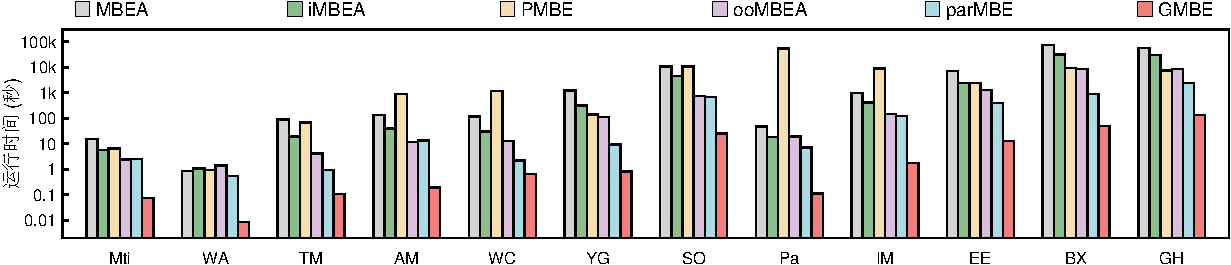
\includegraphics[width=\linewidth]{gmbe/overall}
    % \vspace{0.05in}
	\caption{GMBE整体运行时间评估(对数形式)}
	\label{fig:gmbe_exp_overall}
\end{figure}





\subsection{技术点分解评估}
\label{subsec:gmbe_breakdown}

我们设计了消融实验,分别对GMBE中的枚举节点重用方法、剪枝方法和调度方法等技术点进行了分解评估。

\begin{figure} [H]
	\centering
  \vspace{0.05in}
	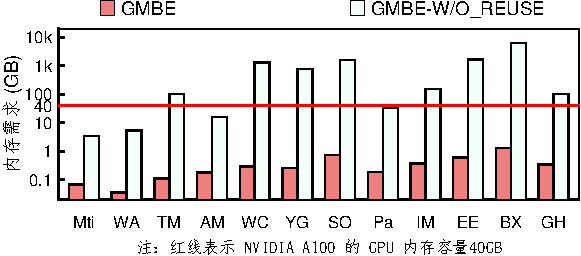
\includegraphics[width=0.8\linewidth]{gmbe/memory.pdf}	
	\vspace{0.05in}
  \caption{枚举节点重用方法的分解评估(对数形式)}
	\label{fig:gmbe_exp_memory}
\end{figure}



\textbf{枚举节点重用方法的效果:} 为了研究第~\ref{subsec:gmbe_memory} 节中枚举节点重用方法的效果,我们设计了变体 GMBE-w/o\_REUSE,根据第~\ref{subsec:gmbe_memory} 节的要求在 GPU 上预先分配内存。我们分别估计了 GMBE 在是否开启枚举节点重用优化方法的情况下使用 \textsf{cudaMalloc} 原语分配的内存需求。这些内存需求包括用于输入二分图和运行时子树的预分配内存。图~\ref{fig:gmbe_exp_memory} 显示,枚举节点重用方法在所有测试数据集上将内存需求显著减少了 49倍--4,819倍。而 GMBE-w/o\_REUSE 在多个数据集上内存需求超出了 A100 GPU 的内存容量,导致无法运行。




\begin{figure}[t]
	\centering
  % \vspace{0.05in}
	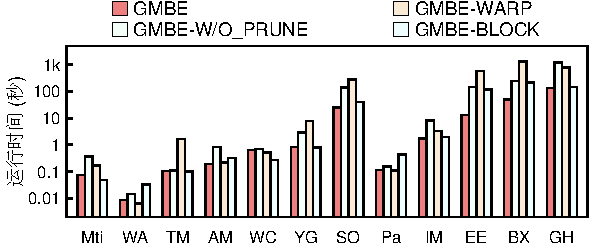
\includegraphics[width=0.8\linewidth]{gmbe/optimization.pdf}	
	% \vspace{0.05in}
  \caption{剪枝方法和任务调度方法的分解评估(对数形式)}
	\label{fig:gmbe_exp_optimization}
\end{figure}

\begin{table}[t]
  % \setlength{\abovecaptionskip}{0cm}  
  \setlength{\belowcaptionskip}{-0.2cm}
	\centering
	\caption{ 剪枝方法使用前后生成的非极大二分团与极大二分团比值比较$\delta/\alpha$}
	\label{tbl:gmbe_prune}
	\begin{center}
    \setlength{\tabcolsep}{2pt}
		\normalsize
    {
			\begin{tabular}{|c|c|c|c|c|c|c|c|c|c|c|c|c|}
				\hline
        \textbf{数据集} &Mti &WA &TM &AM &WC &YG &SO &Pa &IM &EE &BX &GH \\ \hline
        GMBE &9.04 &0.734 &1.63 &12.9 &0.71 &2.11 &89.4 &0.362 &15.5 &4.04 &3.40 &11.1 \\ 
        GMBE-w/o\_PRUNE &66.0 &3.68 &3.88 &53.0 &2.89 &20.1 &174 &1.43 &74.4 &56.0 &27.3 &51.4 \\ \hline
        % \hline
        % \textbf{数据集} &Mti &WA &TM &AM &WC &YG  \\ \hline
        % GMBE &9.04 &0.734 &1.63 &12.9 &0.71 &2.11  \\ 
        % GMBE-w/o\_PRUNE &66.0 &3.68 &3.88 &53.0 &2.89 &20.1  \\ \hline \hline
        
        % \textbf{数据集} &SO &Pa &IM &EE &BX &GH \\ \hline
        % GMBE &89.4 &0.362 &15.5 &4.04 &3.40 &11.1 \\ 
        % GMBE-w/o\_PRUNE &174 &1.43 &74.4 &56.0 &27.3 &51.4 \\ \hline

      \end{tabular}
		}
	\end{center}
  \vspace{-0.1in}
\end{table}

\textbf{剪枝方法的效果:} 为了研究第~\ref{subsec:gmbe_thread_divergence} 节中基于局部邻居数量的剪枝方法的效果,我们设计了一个变体 GMBE-w/o\_PRUNE,仅禁用了 GMBE 的剪枝功能。如图~\ref{fig:gmbe_exp_optimization} 所示,GMBE 总是优于 GMBE-w/o\_PRUNE。这是因为基于局部邻居数量的剪枝方法通过批量比较局部邻居,在控制线程分歧的同时裁剪了大量极大二分团枚举问题的搜索空间。同时,剪枝方法通过比较候选顶点集中相同顶点的局部邻居数量来增强内存访问的连续性。
为了进一步探索剪枝的效率,我们使用$\alpha$表示极大二分团的数量,使用$\delta$表示通过节点检查(算法~\ref{alg:gmbe_stack} 的第18行)生成的被剪枝的非极大二分团的数量。由于$\alpha$对于每个数据集都保持不变,我们使用比值$\delta/\alpha$来表示 GMBE 和 GMBE-w/o\_PRUNE 的剪枝效率,如表~\ref{tbl:gmbe_prune} 所示。
通过比较 GMBE 和 GMBE-w/o\_PRUNE 的$\delta/\alpha$比值,我们观察到所提出的剪枝方法可以在所有测试数据集中避免 48.7\%-92.8\% 的非极大二分团检查。由于极大二分团枚举任务的枚举空间随着极大二分团数量的增加而增长,剪枝技术在更大的数据集中尤为重要。具体而言,剪枝方法将运行时间从 Github 上的 1,191 秒显著减少到 132 秒。

\textbf{负载感知的任务调度方法的效果:} 为研究第~\ref{subsec:gmbe_design_load}节中负载感知的任务调度方法的效果,我们设计了两个变体 GMBE-WARP 和 GMBE-BLOCK,分别采用基于线程束和基于线程块的方案。如图~\ref{fig:gmbe_exp_optimization}所示,在包括 EuALL、Github、BookCrossing、StackOverflow 和 IMDB 在内的大规模实验数据集上,GMBE明显比 GMBE-WARP 和 GMBE-BLOCK 更快,并在其他数据集上花费不到一秒的时间。在大规模实验数据集上,GMBE 的性能更好,因为它动态检测和分区具有重负载的任务,并管理无锁任务队列以在更细粒度上重新平衡工作负载。实验结果显示,在EuALL数据集上,GMBE、GMBE-WARP和GMBE-BLOCK的运行时间分别为13秒、573秒和119秒。由此可见,相较于其他任务调度方法,负载感知的任务调度方法能够显著提升计算性能,尤其在负载不均匀的情况下表现更为突出。
% 结果,GMBE 在 EuAll 上比 GMBE-WARP 快 44.7倍,比 GMBE-BLOCK 快 9.3倍。

\begin{figure} [H]
	\centering
  \subfloat[StackOverflow]	{
		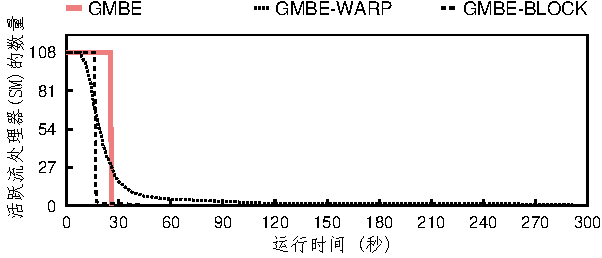
\includegraphics[width=0.47\linewidth]{gmbe/load_balance_so.pdf}
		\label{fig:balance_stackoverflow}
	} 
	\subfloat[EuAll]{
		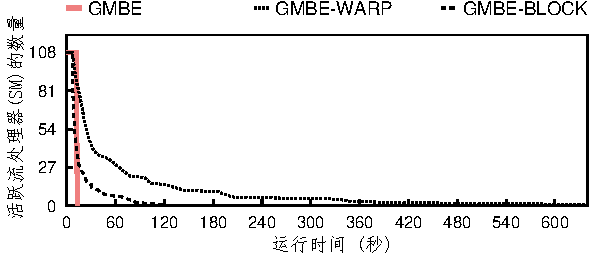
\includegraphics[width=0.47\linewidth]{gmbe/load_balance_ea.pdf}
		\label{fig:balance_euall}
	} \\
	\subfloat[BookCrossing]	{
		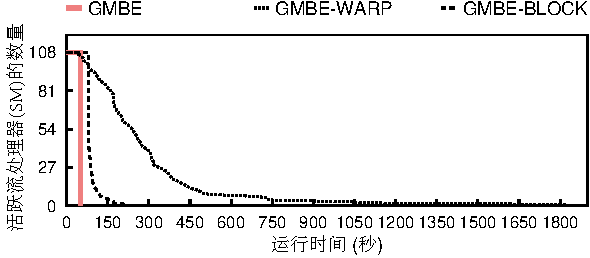
\includegraphics[width=0.47\linewidth]{gmbe/load_balance_bx.pdf}
		\label{fig:balance_bookcrossing}
	}	
  \subfloat[Github]	{
		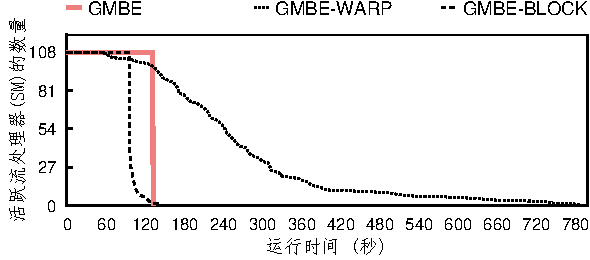
\includegraphics[width=0.47\linewidth]{gmbe/load_balance_gh.pdf}
		\label{fig:balance_github}
	}

	\caption{不同调度方法中SM上的运行时负载比较}

	\label{fig:gmbe_exp_balance}
\end{figure}



为了更深入地探究 GPU 上进行极大二分团枚举 面临的负载不平衡问题,我们记录了在运行 GMBE、GMBE-WARP 和 GMBE-BLOCK 时GPU内活跃流处理器数量随着运行时间的变化情况。图~\ref{fig:gmbe_exp_balance} 对比展示了在StackOverflow、EuALL、BookCrossing 和 Github 数据集上 SM 的运行负载。由于存在工作负载不平衡,一些负载较轻的 SM 可能会提前完成并等待那些负载较重的 SM,这将增加整体运行时间。由于负载不平衡问题的存在,GMBE-WARP 中活跃的 SM 数量迅速减少,因而表现最差。相比之下,GMBE-BLOCK 获得了更好的性能,因为它可以为每个工作负载分配更多资源(即一个线程块而非一个线程束),从而减少了等待具有最重负载的 SM 的时间。然而,GMBE-BLOCK仍然存在不足,因为极大二分团枚举问题的工作负载可能严重不平衡。例如,在 EuALL 数据集上,超过 80\% 的 SM(86 个 SM / 108 个 SM)浪费了超过 80\% 的运行时间(98 秒 / 118 秒)在等待最慢的 SM。相比之下,GMBE 总是能够实现最佳性能,因为它能够在最细粒度上工作,使得每个 SM 大致同时完成其工作。在 BookCrossing 数据集上,甚至在 GMBE-BLOCK 的活跃 SM 数量开始减少之前,GMBE 就已经完成了运算,因为它在每个 SM 中激活了所有的线程束,而相比之下,GMBE-BLOCK 在运行时可能只使用了每个 SM 中的一小部分线程束。



% 图~\ref{fig:gmbe_load_example}展示了在简单负载均衡方案下,在GPU上进行极大二分团枚举表现出的负载不均问题。具体而言,首先,在我们的最终解决方案GMBE的基础上,我们应用G$^2$Miner算法中将每个顶点生成的枚举子树分配给GPU上的一个线程束来独立执行的任务调度方案,形成变种GMBE-WARP。随后,我们在BookCrossing数据集上运行GMBE-WARP,并记录了GPU内活跃流处理器数量随着运行时间的变化图。实验结果显示,该算法的总运行时间为1,822秒。当程序运行至20\%时(即364秒),活跃的流处理器仅有22个,占总数108个的20\%。这意味着在整个运行过程中,超过80\%的流处理器(86个SMs / 共108个SMs)将耗费80\%的运行时间(1,458秒 / 共1,822秒)等待最慢的一个子枚举树的计算。因此,现有的方法不能满足极大二分团枚举算法在GPU上的负载均衡需要,我们有必要实现更细粒度的负载均衡。



\subsection{敏感性测试}
\label{subsec:gmbe_sensitivity}


\begin{figure} [H]
	\centering
  \vspace{0.1in}
	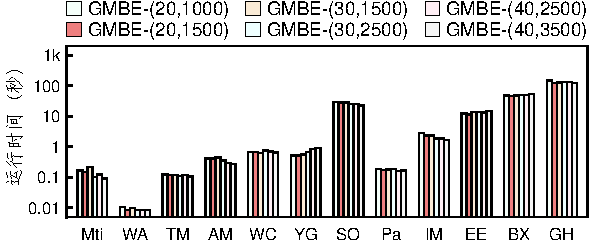
\includegraphics[width=0.8\linewidth]{gmbe/cost_function.pdf}	
	\vspace{0.1in}
  \caption{负载感知任务调度下阈值设置 (对数形式)}
	\label{fig:gmbe_exp_cost}
\end{figure}


\textbf{负载感知任务调度阈值对性能的影响:} 为了探究在~\ref{subsec:gmbe_design_load}节中阈值 $bound\_height$ 和 $bound\_size$ 的有效配置,我们设计了多个变种 GMBE-$(m, n)$,其中$m$ 和 $n$ 分别代表 $bound\_height$ 和 $bound\_size$。我们总是设置 $m$ 大于 $n^2$,因为我们知道  $|L|\times|C|$ 始终大于或等于 $(min\{|L|,|C|\})^2$。阈值的选择是并行粒度和同步开销之间的权衡。我们需要更小的阈值来在更细的粒度上平衡工作负载。然而,阈值不应该过小。否则,我们将不得不处理更多带有巨大同步开销的任务。图~\ref{fig:gmbe_exp_cost} 表明,在大多数情况下,变种 GMBE-(20, 1500) 在运行时间上优于其他变种。因此,GMBE默认应用这种配置。


\begin{figure} [H]
	\centering
  \vspace{0.1in}
	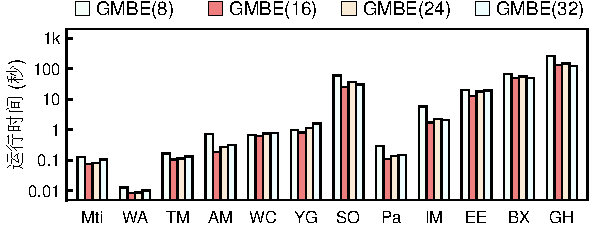
\includegraphics[width=0.8\linewidth]{gmbe/parameters.pdf}	
	\vspace{0.1in}
  \caption{参数\textsf{WarpPerSM}设置 (对数形式)}
	\label{fig:gmbe_exp_config}
\end{figure}

\textbf{每个流处理器中线程束数量的影响:} 为确定第~\ref{subsec:gmbe_design_load} 节中 PT 模型中参数 \textsf{WarpPerSM},我们设计了将 \textsf{WarpPerSM} 设置为 8、16、24 和 32 的不同变种。参数\textsf{WarpPerSM} 的选择是并行性和每个线程束资源之间的权衡。直觉上,我们希望 \textsf{WarpPerSM} 更大,以便可以并行运行更多的极大二分团枚举任务。然而,\textsf{WarpPerSM} 不应该过大,因为每个流多处理器中的计算资源(例如寄存器)是有限的。较大的 \textsf{WarpPerSM} 可能会降低 GMBE的性能,因为每个线程束将拥有更少的资源来运行极大二分团枚举任务。图~\ref{fig:gmbe_exp_config} 显示,在大多数大规模数据集(如 BookCrossing、StackOverflow、IMDB、DBLP 和 EuAll)中,变种 GMBE-16的性能优于其他变种高达 3.83倍。此外,由于其广泛的枚举空间需要更多线程束并行枚举极大二分团,GMBE-16在 Github 上比 GMBE-32慢 0.94倍。考虑到在大多数情况下的效率,GMBE默认将 \textsf{WarpPerSM} 设置为 16。

\begin{figure} [H]
	\centering
	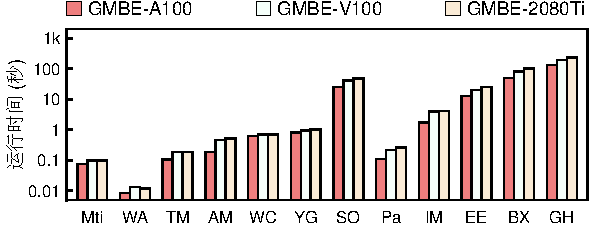
\includegraphics[width=0.8\linewidth]{gmbe/diffgpus.pdf}	
	\vspace{0.1in}
  \caption{GMBE在不同型号GPU上的适用性(对数形式)}
	\label{fig:gmbe_exp_diff}
\end{figure}

\textbf{在不同GPU上的适用性:} 为了探究GMBE在不同GPU上的适用性,我们分别在NVIDIA A100 GPU(108个流多处理器,40 GB全局内存)、NVIDIA V100 GPU(80个流多处理器,32 GB全局内存)~\cite{NVIDIA-V100}和NVIDIA 2080Ti GPU(68个流多处理器,11 GB全局内存)~\cite{NVIDIA-2080Ti}上对GMBE进行评估。图~\ref{fig:gmbe_exp_diff} 显示GMBE在所有三种GPU上都表现出了适用性。GMBE-A100 稍微快于 GMBE-V100 和 GMBE-2080Ti,因为A100 GPU包含比其他GPU更多的计算资源。

\begin{figure} [H]
	\centering

	\subfloat[BookCrossing]	{
		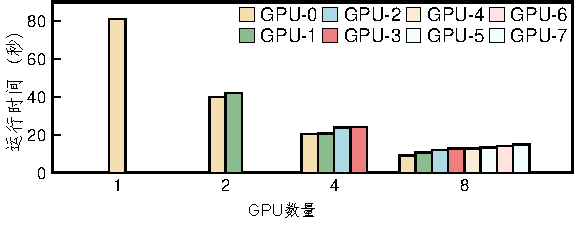
\includegraphics[width=0.8\linewidth]{gmbe/multi_scalability_BookCrossing.pdf}
		\label{fig:scalability_bookcrossing}
	} \\

	\subfloat[Github]	{
		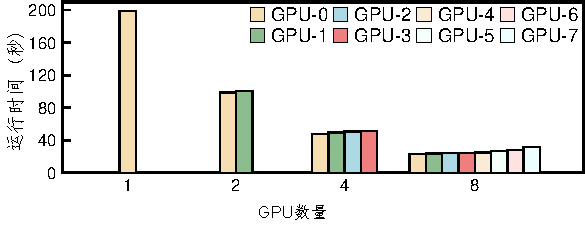
\includegraphics[width=0.8\linewidth]{gmbe/multi_scalability_Github.pdf}
		\label{fig:scalability_github}
	}

	\caption{GMBE在多GPU环境下的可扩展性}

	\label{fig:gmbe_exp_scale}

\end{figure}

\textbf{多GPU环境下的可扩展性:} 为了探究GMBE在多GPU环境下的可扩展性,我们在一台配备了8个NVIDIA V100 GPU的机器上进行了实验。为了优化GMBE以适应多GPU配置,我们将问题分解为多个独立的子问题,总运行时间由运行时间最长的子问题决定。 图~\ref{fig:gmbe_exp_scale} 显示,随着GPU数量的增加,GMBE在Github和BookCrossing数据集上呈线性扩展,因为每个GPU几乎同时完成其执行。在多个GPU的帮助下,GMBE能够在31秒内枚举出Github数据集中超过5500万个极大二分团,相较于96核CPU机器上最先进的并行极大二分团枚举算法ParMBE(即2411秒),性能提升了77倍。

\section{本章小结}

本章介绍了针对极大二分团枚举问题的高效GPU解决方案GMBE。首先,针对GPU上运行极大二分团枚举算法所带来的内存短缺问题,我们提出了基于枚举节点重用的迭代方法,通过重用根节点内存,减小动态内存分配带来的内存开销。其次,针对现有剪枝方法引入的线程分歧问题,本章提出了局部邻居数量感知的剪枝方法,通过对中间结果的批量比较,在实现高效剪枝性能的同时缓解了线程分歧问题。再次,针对现有方法难以实现极大二分团枚举任务负载均衡的问题,本章提出了负载感知的任务调度方法,动态识别并拆分具有高负载的任务,实现细粒度的任务调度。最后,我们结合上述技术,实现了GMBE算法。实验结果充分证明了GMBE算法在GPU上的高性能以及本章中所有方法的具体作用。